\documentclass{MMCStyle}
\usepackage[minted, multicol]{MyTemplate} % 如果要用minted的话，要自己加-shell-escape
% \usepackage{MyTemplate}
\usepackage{zhlipsum}
\usepackage{lipsum}
\usepackage[version=4]{mhchem}

\bianhao{MC1111111}
\tihao{X}
\timu{起啥题目呢}
\keyword{你觉得什么关键词比较合适；不知道；那就乱写吧}
% \bibliographystyle{gbt7714-numerical}
\addbibresource{ref.bib}

\graphicspath{{./images/}}


\makeatletter
\newcommand{\mysupercite}[1]{\textsuperscript{\cite{#1}}} % 这种做法虽然有点丑陋，但是胜在简单易行。因为丑陋，所以没放自定义宏包`MyTemplate`里
\makeatother

\setcounter{tocdepth}{2} % 目录深度，自己调

\renewcommand{\tabularxcolumn}[1]{m{#1}} % 1. 让所有X列垂直居中
\newcolumntype{C}{>{\centering\arraybackslash}X} % 2. 定义水平居中的X列

\begin{document}
% \nocite{*}

% 摘要默认小四号字 \zihao{-4} ，如果内容比较多一页放不下的话，自己去 `MMCStyle.cls` 里改字号，比如改成 \zihao{5} 。
\begin{abstract}

摘要开始。

\textbf{针对问题一：}\lipsum[1]

\textbf{针对问题二：}\zhlipsum[2]

\textbf{针对问题三：}为什么还要写摘要。

我不想写摘要，摘要要认真写。% 注意\end{abstract}前面不能空行
\end{abstract}



% 取消目录页码
\tableofcontents\newpage
\clearpage
\pagenumbering{arabic}
\pagestyle{fancy}
% 恢复默认的页面样式



\section{问题重述}

\subsection{问题背景}

\zhlipsum[4]

\subsection{问题提出}% 不一定非要按照这个格式，前面怎么写自行参考多篇优秀论文，但实际上是有自由度的。

阿巴阿巴。

\begin{description}
  \item[\bfseries 问题一]随便写啦。
  \item[\bfseries 问题二]也许吧。
  \item[\bfseries 问题三]不会，靠建模手了。
  \item[\bfseries 问题四]\LaTeX{}编译缓慢没办法，背负着历史的包袱。感兴趣的话可以试试 Typst ，秒出 PDF 。
\end{description}

\section{问题分析}

\subsection{总体分析}

\lipsum[4]

\subsection{问题一的分析}

\zhlipsum[2]

\subsection{问题二的分析}

问题二的分析已经被概括为 $\ee^{\ii \theta} = \cos\theta + \ii \sin\theta$ 了，或者 $\displaystyle\dv{}{x} \e^x = \ee^x = \exp\lr(x)$ 。

\subsection{问题三的分析}

\lipsum[4]

\section{模型假设}

为了我的叽里咕噜看上去高级一点，我们做了如下假设：

\begin{enumerate}
  \item 我觉得 Markdown 不好用。
  \item 我觉得 \LaTeX 不是那么好用。
  \item 我正在学习 Typst 。
  \item Word 采用的数学字体的排版效果看上去确实没有 Computer Modern 或者 Latin Modern 的好看。
\end{enumerate}



\section{符号说明}

\inline{siunitx} 宏包和 \inline{physics} 宏包在 \inline{qty} 上的冲突也是出了名的，但是我就是不用 \inline{physics2} 宏包。

\begin{table}[!htbp]
\centering
\caption{快看，这是第一个表格的 caption}
\label{table:symbols}
\footnotesize
\begingroup
\begin{tabularx}{\textwidth}{@{}XX@{}}
\toprule
\textbf{表头} & \textbf{标头} \\
\midrule
你好 & 世界 \\
$\partial D$ & $\mathbb{I}\lr(x>0)$ \\
\bottomrule
\end{tabularx}
\endgroup
\vspace{0.4em}

\noindent\footnotesize{\textbf{符号规范说明：}写作要规范一点，直立体表达一个变量，斜体是隐式乘法。}
\end{table}



\section{问题一模型的建立与求解}

\ce{Na+} 在我创办的期刊上指出：“拒绝半桶水的水平”\mysupercite{book01}。在使用单位 $\unit{\kilo\m\per\s}$ 下，一个不知名的式子
\[
  \zeta_{\mathrm{op}} + \e = \ii
\]
其中， $\e$ 为自然常数。

我\mysupercite{deepseek}曾提到： AI 并非民事行为能力人，只不过是一个高级点的搜索引擎，不应该放进参考文献的条目里。

\lipsum[3]

\subsection{副标题自己定}

$\unit{\m\per\s}$ 和 $\SI{100e-6}{\m}$ 好看。

\zhlipsum[3]

\begin{table}[!htbp]
\centering
\caption{加油}
\label{table:好看的}
\begin{tabular}{ccc}
\toprule
三 & 三 & \textbf{三} \\
\midrule
线 & 线 & 线 \\
表 & 表 & 表 \\
\bottomrule
\end{tabular}
\end{table}

\cref{table:好看的} 是好看的。

\begin{figure}[!htbp]
\centering
\begin{minipage}[b]{0.48\textwidth}
\centering
\footnotesize

\includegraphics[width=\textwidth]{无标题1.png}
\caption{无标题 1}
\label{figure:untitled 1}
\end{minipage}
\hfill
\begin{minipage}[b]{0.48\textwidth}
\centering
\footnotesize
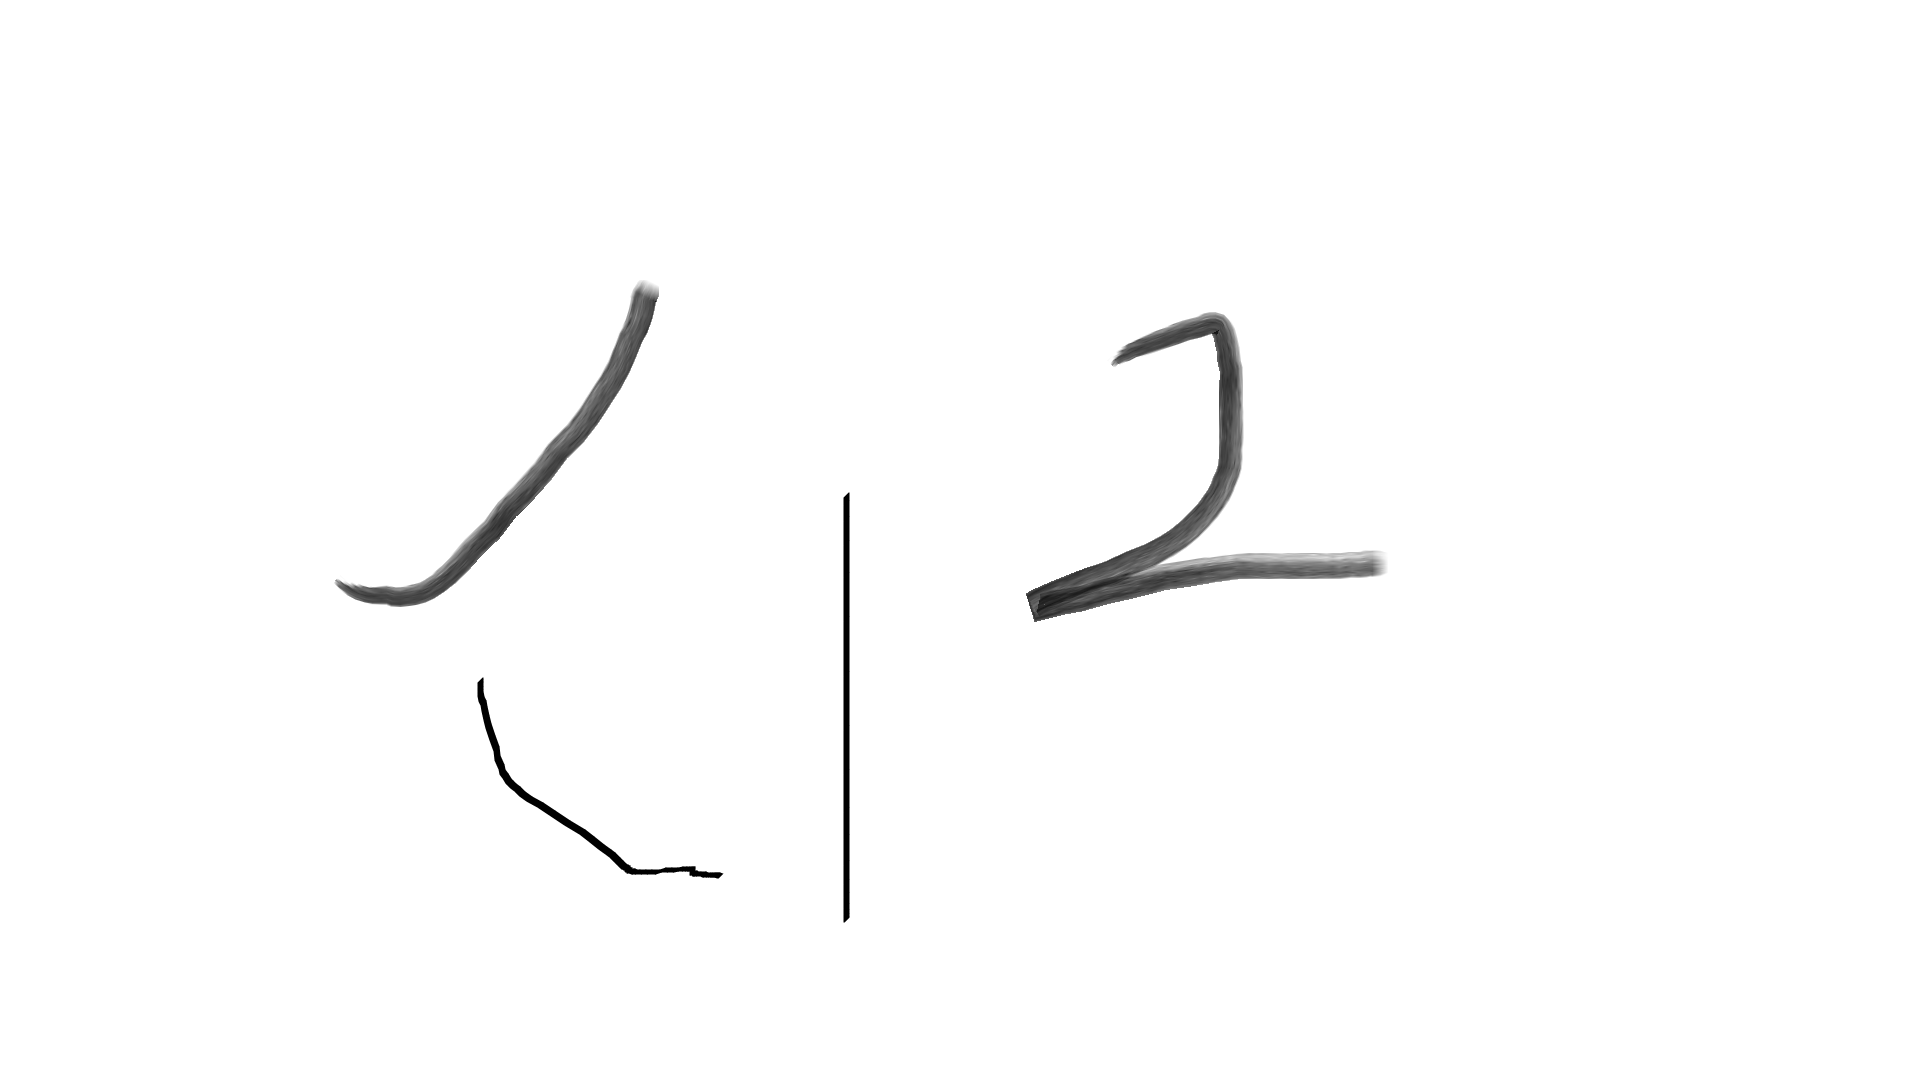
\includegraphics[width=\textwidth]{无标题2.png}
\caption{无标题 2}
\label{figure：untitled 2}
\end{minipage}
\end{figure}

\zhlipsum[6]

如\cref{figure:untitled 1} 所示，阿巴阿巴。

\begin{equation}
\sin[2]\theta + \cos^2\theta = 1
\end{equation}

终于写完了，制作不易，觉得有用的话记得点个 \inline{Star} 。

\subsubsection{快来快来数一数，二四六七八}

\lipsum[5]

\begin{figure}[!htbp]
\centering

\includegraphics[width=0.7\textwidth]{无标题1.png}
\caption{懒得写了}
\label{figure:你好压}
\end{figure}

如\cref{figure:你好压} 所示，我已经亚历山大了。

\subsubsection{Bad 略略略}

\zhlipsum[2]

\subsection{计入 PDF 书签的章节命令尽量只用纯文本 plain text}

\section{下划线最容易踩坑了，吗}

长 \inline{my\_bot} 得 \inline{is\_true} 好 \inline{不} 丑。

\begin{equation}\label{equation:important}
  a + b = c
\end{equation}

\subsection{问题一小结}

后面\cref{equation:important} 不给那么详细了。


\section{问题二的模型建立与求解}

\subsection{略略略}

已。

\subsection{略}

经

\subsubsection{没写}

完了。网络\mysupercite{web01}里面啥都有。

\section{模型的优缺点分析与优化}

章节结构随便改，也没有谁说优缺点\mysupercite{paper01}分析是必须有的。

\subsection{问题一模型的分析与改进}

\subsubsection{也许已经很完美了吧}

Good 好。

% \clearpage
\phantomsection
\addcontentsline{toc}{section}{参考文献}
% \bibliography{ref}
\printbibliography[title={参考文献}] % 输出列表

\appendix

\section*{附录}

% \section*{\LARGE 附录}\addcontentsline{toc}{section}{附录}

柯西（可惜）附件 4 \footnote{MathorCup 数学应用挑战赛人工智能工具使用规定（试行）}第四节要求不被遵守，本文将使用的 AI 放入了参考文献的条目中。

\inline{minted} 提供的参数请自行检索，例如 \inline{breaklines} 。

想用不需要 \inline{-shell-escape} 的 \inline{listings} 也行，看个人方便程度和要求以及喜好。

\section{单栏示例}

\begin{minted}[fontsize=\tiny,linenos,breaklines,frame=single]{typst}
#import "@preview/physica:0.9.8": *
#import "@preview/theorion:0.4.1": *
#import cosmos.fancy: *
// #import cosmos.rainbow: *
// #import cosmos.clouds: *
#show: show-theorion


#let hblank = { $wide wide wide$.body }
#let sgn = math.op("sgn")
#let my-example = definition-box.with(breakable: true)
#let my-proof = corollary-box.with(breakable: true)
// 虚数单位i
#let ii = { $upright(i)$.body }
// 自然常数e
#let ee = { $upright(e)$.body }
#show math.equation: set text(features: ("cv01",))
// 定义可跨页横线，支持自定义样式
#let crosspage-hline(..args) = {
  // 提取 stroke 参数，默认为 1pt 黑线
  let stroke = args.named().at("stroke", default: 1pt + orange)

  // 取消首行缩进
  set par(first-line-indent: 0pt)

  // 绘制横线，使用 box 确保宽度准确
  box(
    width: 100%,
    height: 0.6em, // 类似 baseline=-0.6ex 的垂直调整
    align(horizon, line(length: 100%, stroke: stroke)),
  )

  parbreak()
}/*
 // 使用示例
 #crosspage-hline()
 #crosspage-hline(stroke: 2pt + red)
 #crosspage-hline(stroke: (thickness: 1pt, paint: blue, dash: "dashed")) */


#import "@preview/xarrow:0.4.0": xarrow
#let xlongequal = xarrow.with(sym: sym.eq)
#let dcase(title: none, body) = {
  grid(
    columns: (auto, 1fr),
    gutter: 1em,
    box(width: 2em, height: 2em, fill: rgb("#e8e8e8"), radius: 50%, align(center + horizon, strong(
      $ note.grace $,
    ))),
    [
      === #title
      #body
    ],
  )
}
#let alternative-solution(title: "Alternative Solution", body) = {
  grid(
    columns: (auto, 1fr),
    gutter: 1em,
    box(width: 1em, height: 1em, fill: rgb("#779177"), radius: 10%, align(center + horizon, strong(
      $ crossmark $,
    ))),
    [
      === #title
      #body
    ],
  )
}

#set page(
  // 以A4纸为例，你可以改成其他尺寸或自定义width, height
  paper: "a4",
  // 让左右、上下边距都等于页面宽/高的7.5%，从而使版心占85%
  margin: (x: 7.5%, y: 7.5%),
)

// 填充底色
#set page(
  fill: rgb("#FFF2E2FF"),
)

#set document(
  title: "一些有跳跃间断点的函数的原函数",
  author: "DevlinNul",
)
#set par(justify: true)
#title()

= 一些约定

本文在求原函数时不会显式地写 $+C$ 。

本文探讨的积分是勒贝格积分意义下的，即只考虑函数几乎处处（almost everywhere，即a.e.）的行为，而忽略函数在零测集上的行为。

本文中限制函数的定义域只能是一个区间。

本文采用的符号函数的定义为
$
  sgn x colon.eq cases(
    1 & quad "if" x > 0,
    0 & quad "if" x = 0,
    -1 & quad "if" x < 0
  )
$

本文中，分段常数函数指定义在一个区间上，导数几乎处处为零的函数。如定义在 $RR$ 上的 $sgn x, ceil(x), floor(x), round(x), 0, 1, 2, x-arctan(tan x)$ 等等（ $x-arctan(tan x)$ 作延拓处理，跳跃间断点处的函数值取某一个单侧极限值），其中，前四者分别称为“符号函数”、“向上取整函数”、“向下取整函数”、“四舍五入函数”。注意分段常数函数是包括了常数函数的。后文中，我们假定函数的跳跃间断点总能归结为分段常数函数的跳跃间断点。我们断言，一个实变函数的第一类间断点组成的集合一定是至多可数的，因而一定是零测集。

在求原函数的过程中，将分段常数函数视为常数处理的步骤会用 $eq.star$ 标明。

= 正文

对于间断点仅含有第一类间断点（可去间断点和跳跃间断点）的函数，其定积分总是连续的。

但我们在求其不定积分时，中间步骤可能由于将分段常数函数视为常数提取到积分号外之类的不等价的操作（如将 $sgn(x)$ 当做常数随意地提取到积分号外）导致最后算出来的结果可能仅在局部成立，而在全局不成立。在几乎处处的意义下，求原函数时我们不要求原函数 $F$ 在被积函数 $f$ 的跳跃间断点上满足 $F'=f$ ，只需要这个式子几乎处处成立即可。所以标准的做法是在被积函数的每一个连续区间里分别积分，在这样的每一个连续区间里，分段常数函数恰好分别是该区间上的常数；但这样得到的原函数的形式是分段的，不一定是定义域（限定为一个区间）上的绝对连续函数，从而无法利用牛顿--莱布尼茨公式（牛莱公式），这不是我们想要的。若我们需要得到绝对连续的原函数，还需要调整各个区间的常数，使得不同区间上得到的结果拼接（后文将称之为修正）成定义域上的绝对连续函数（可去间断点进行延拓处理，即补充定义函数值为极限值）。

我们求不定积分时通常总是希望得到绝对连续的原函数，使得牛莱公式可用。既然标准的做法难以得到绝对连续的原函数，那我们就不必严格地按照标准做法去做。由于分段常数函数在不同的连续区间上的函数值的差值总是常数，所以我们逐区间积分再修正与这种做法是等效的：在定义域上将分段常数函数视为常数，得到的结果再进行连续性修正。我们对此给出简要的说明。

#my-proof(title: "等效性证明")[
  设 $A, D_1, D_2, dots, D_n$ 是 $D$ 的一个划分，即
  $
    cases(
      limits(union.big)_(i=1)^(n) D_i union A = D,
      forall i in NN^+ \, forall j in NN^+ comma i eq.not j ==> D_i inter D_j = emptyset,
      forall i in NN^+ comma A inter D_i = emptyset
    )
  $
  并且 $A$ 的测度 $mu(A) = 0$ ， $D_i$ 均为区间。
  假设分段常数函数 $p(x)$ 满足
  $
    p(x) = cases(
      p_1 comma quad x in D_1,
      p_2 comma quad x in D_2,
      dots.v,
      p_n comma quad x in D_n
    )
  $
  其中 $p_i$ 为某一实数， $n in NN^+$ 或者 $n->+oo$ 。

  我们之所以能够将 $p(x)$ 的取值列出来，是因为我们断言了：任何实变函数的第一类间断点组成的集合一定是至多可数的。

  由于我们假定了研究的函数的跳跃间断点总能归结为分段常数函数的跳跃间断点，于是对于 $D$ 上的连续函数 $f$，我们研究
  $
    integral p(x) dot f(x) dif x
  $
  的计算。之所以将被积函数直接写成乘积的形式，是因为积分运算的线性性满足
  $
    integral c f(x) dif x = c integral f(x) dif x, c "为某一实数"
  $

  于是在忽略原函数的绝对连续性的前提下
  $
    integral p(x) f(x) dif x & = cases(
                                 p_1 integral f(x) dif x comma quad x in D_1,
                                 p_2 integral f(x) dif x comma quad x in D_2,
                                 dots.v,
                                 p_n integral f(x) dif x comma quad x in D_n
                               ) \
                             & = p(x) integral f(x) dif x
  $

  于是在不考虑原函数的绝对连续性的前提下，分段常数函数可以视为常数自由进出积分号。而分段积分的方法最后需要进行连续性修正，将分段常数函数视为常数的做法最后也需要进行连续性修正，所以我们可以直接采取后者，以期简化运算。
]
需要指出的是，牛莱公式要求原函数是绝对连续的。但是我们的拼接操作最多只能保证得到的结果是连续的，是否绝对连续是由区间上函数的行为决定的。所以，我们只说进行连续性修正而不是绝对连续性修正。

下面给出一些实例。

#my-example(title: [求 $display(integral sgn x dif x)$ ])[
  先将 $sgn x$ 视为常数，于是 $ integral sgn x dif x eq.star sgn x integral dif x = x sgn x $

  然后检查得到的原函数的连续性。

  记 $F colon.eq x sgn x$ 。由于 $sgn x$ 有唯一间断点 $x = 0$ ，而
  $
    display(lim_(x->0^+)F(x) &= 0 times 1 = 0) \
    display(lim_(x->0^-)F(x) &= 0 times (-1) = 0)
  $
  于是 $display(lim_(x->0^+)F(x) = lim_(x->0^-)F(x))$ ，所以 $F$ 是连续的，无需连续性修正。
]

#my-example(title: [求 $display(integral ee^(-abs(x)) dif x)$ ])[
  $
    integral ee^(-abs(x)) dif x & = integral ee^(- sgn(x) dot x) dif x = integral (ee^(- sgn x))^x dif x \
                                & eq.star (ee^(- sgn x))^x/(ln(ee^(-sgn x))) = ee^(-abs(x))/(-sgn x)
  $
  记 $display(F(x) = ee^(-abs(x))/(-sgn x))$ ，则
  $
    lim_(x->0^-) F(x) & = 1 \
    lim_(x->0^+) F(x) & = -1
  $
  取
  $
    h(x) & = -display(lim_(x->0^+) F(x) - lim_(x->0^-) F(x))/2 dot sgn(x) \
         & = sgn x
  $
  于是
  $
    overline(F)(x) = -ee^(-abs(x))/(sgn x) + sgn x
  $
  则 $overline(F)(x)$ 在 $x=0$ 处有可去间断点，可以补充定义 $overline(F)(0) = 0$ ，即可得到延拓到 $RR$ 的 $overline(F)(x)$ 。
  值得注意的是，将 $overline(F)(x)$ 写成 $-ee^(-abs(x)) dot sgn x + sgn x$ ，即
  $
    overline(F)(x) = sgn x dot (1 - ee^(-abs(x)))
  $
  可以自动得到 $RR$ 上的连续函数。
]

#my-proof(
  title: [证明：设 $A(x), B(x)$ 在 $x=0$ 的一个邻域上有定义， $display(F(x) = A(x)/(sgn x) + B(x))$ ，满足 $F(x)$ 在 $x=0$ 处有可去间断点，且 $display(B(0) = lim_(x->0)F(x))$ ，则延拓为在 $x=0$ 的一个邻域上连续的 $F(x)$ 为 $overline(F)(x) = A(x) dot sgn x + B(x)$ ],
)[
  由于 $F(x)$ 在 $x=0$ 处有可去间断点，故
  $
    lim_(x->0) F(x) colon.eq L
  $
  而 $overline(F)(0) = B(0) = L$ 。于是
  $
    lim_(x->0) F(x) = overline(F)(0)
  $
  由于 $forall x eq.not 0$ ，有 $display(sgn x = 1/(sgn x))$ ，于是
  $
    F(x) equiv overline(F)(x) , quad forall x eq.not 0
  $
  综上， $overline(F)(x)$ 为 $F(x)$ 在 $x=0$ 的一个邻域上的连续延拓。

  #crosspage-hline()

  但实际上，即便 $display(B(0) eq.not lim_(x->0) F(x))$ ，记 $display(L colon.eq lim_(x->0)F(x))$ ，也可以令 $hat(F)(x) colon.eq A(x)/(sgn x) + B(x) + L - B(0)$ ，则 $hat(F)(x)$ 为满足上述证明中的 $F(x)$ ，因为 $L - B(0)$ 为确定的某一常数。

  而在不定积分中，一个原函数加上任意的实数得到的函数属于原函数族，故如果求原函数时得到题设的形式，可以直接将 $sgn x$ 从分母移到分子。
]


\end{minted}

\section{双栏示例}

\begingroup
\setlength{\columnseprule}{0pt}
\begin{multicols}{2}
\begin{minted}[fontsize=\tiny,linenos, numbersep=0.2em,frame=single]{python}
# -*- coding: utf-8 -*-
from janim.imports import *


class Introduction(MyTimeline, SubtitleTemplate2):
    AUDIOS_SUBDIR = "Introduction"
    name = "Introduction"

    def construct(self):
        super().construct()
        dot_a = Dot(LEFT * 5, color=RED)
        text_a = TypstMath(R"A", color=RED)
        dot_b = Dot(RIGHT * 1, color=BLUE)
        text_b = TypstMath(R"B", color=BLUE)
        auxiliary_circle = Circle(color=WHITE)
        vec_a = np.array((1, 0, 0))

class Introduction(MyTimeline, SubtitleTemplate2):
    AUDIOS_SUBDIR = "Introduction"
    name = "Introduction"

    def construct(self):
        super().construct()
        dot_a = Dot(LEFT * 5, color=RED)
        text_a = TypstMath(R"A", color=RED)
        dot_b = Dot(RIGHT * 1, color=BLUE)
        text_b = TypstMath(R"B", color=BLUE)
        auxiliary_circle = Circle(color=WHITE)
        vec_a = np.array((1, 0, 0))

class Introduction(MyTimeline, SubtitleTemplate2):
    AUDIOS_SUBDIR = "Introduction"
    name = "Introduction"

    def construct(self):
        super().construct()
        dot_a = Dot(LEFT * 5, color=RED)
        text_a = TypstMath(R"A", color=RED)
        dot_b = Dot(RIGHT * 1, color=BLUE)
        text_b = TypstMath(R"B", color=BLUE)
        auxiliary_circle = Circle(color=WHITE)
        vec_a = np.array((1, 0, 0))

class Introduction(MyTimeline, SubtitleTemplate2):
    AUDIOS_SUBDIR = "Introduction"
    name = "Introduction"

    def construct(self):
        super().construct()
        dot_a = Dot(LEFT * 5, color=RED)
        text_a = TypstMath(R"A", color=RED)
        dot_b = Dot(RIGHT * 1, color=BLUE)
        text_b = TypstMath(R"B", color=BLUE)
        auxiliary_circle = Circle(color=WHITE)
        vec_a = np.array((1, 0, 0))
\end{minted}
\end{multicols}
\endgroup

\end{document}
